%======================================================================
\subsection{UI step C: built (23 Oct 2026), for your check}\label{sec:ui-stepC-built}
%======================================================================

\paragraph{Your answers (22--23 Oct).} All nine recommendations in section~\ref{sec:ui-stepC} were accepted. On
question~7 you added: the vault homepage replaces the stock Start page. Also accepted with them: the pack sets
\emph{Rotation mode} to \emph{Drag at cursor} (\code{View/RotationMode}~=~1), the toolbar restore after
FreeCAD-Ribbon runs once per workbench, and toolbars are locked (\code{General/LockToolBars}), as C1's risk note
asked. Everything below is Python in \file{src/Mod/BruceWorx/}, each part with its own switch on Preferences
$\rightarrow$ BruceWorx, on by default; the only C++ line is the notification fix in item~7.

\begin{figure}[!htbp]
\centering
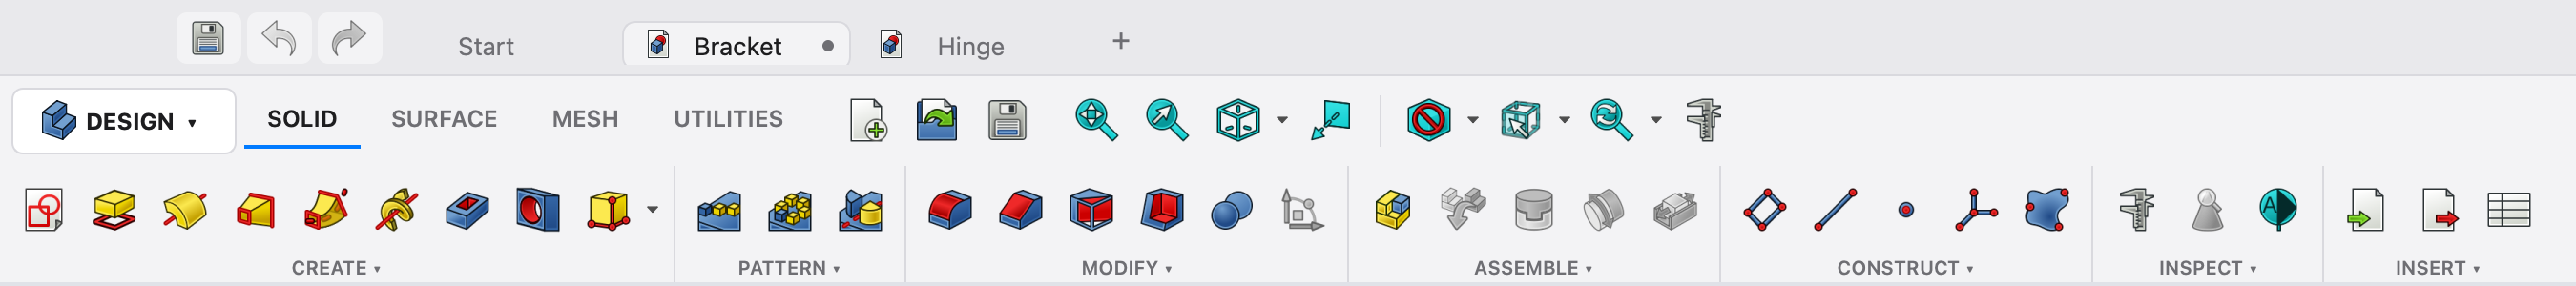
\includegraphics[width=\linewidth]{fig/ui_stepC_built_light.png}\\[4pt]
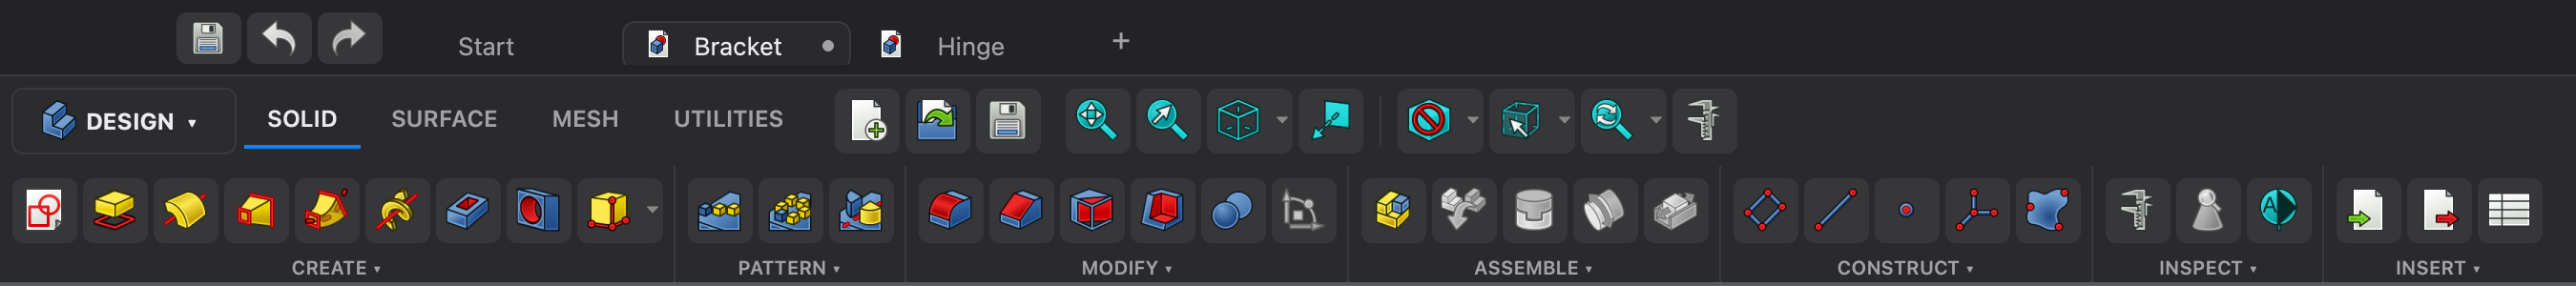
\includegraphics[width=\linewidth]{fig/ui_stepC_built_dark.png}
\caption{Step C as built, captured from the build (light, then dark; the left two thirds of the window). Row~1
is the macOS title bar (C4): the traffic lights (not in a Qt capture) sit left of save, undo and redo, then the
document tabs with the modified dot and \emph{+}; the search field is at the right end
(figure~\ref{fig:stepC-built-menus}). Row~2: the workspace button and its tabs (C2), then File and View.
Row~3: the \textsc{Solid} tab's groups with their captions (C1).}
\label{fig:stepC-built}
\end{figure}

\begin{figure}[!htbp]
\centering
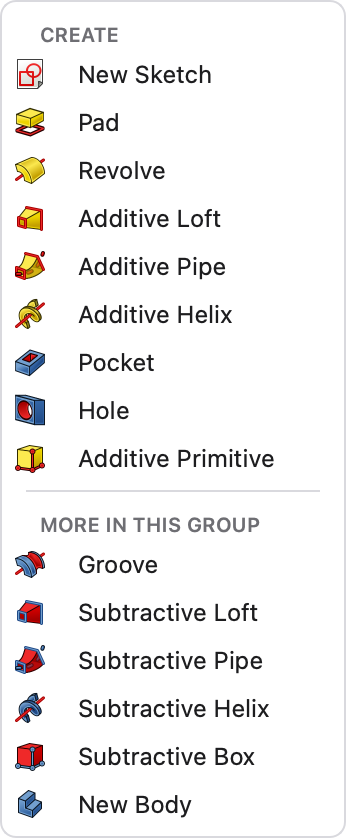
\includegraphics[height=7.2cm]{fig/ui_stepC_built_caption.png}\hspace{8mm}
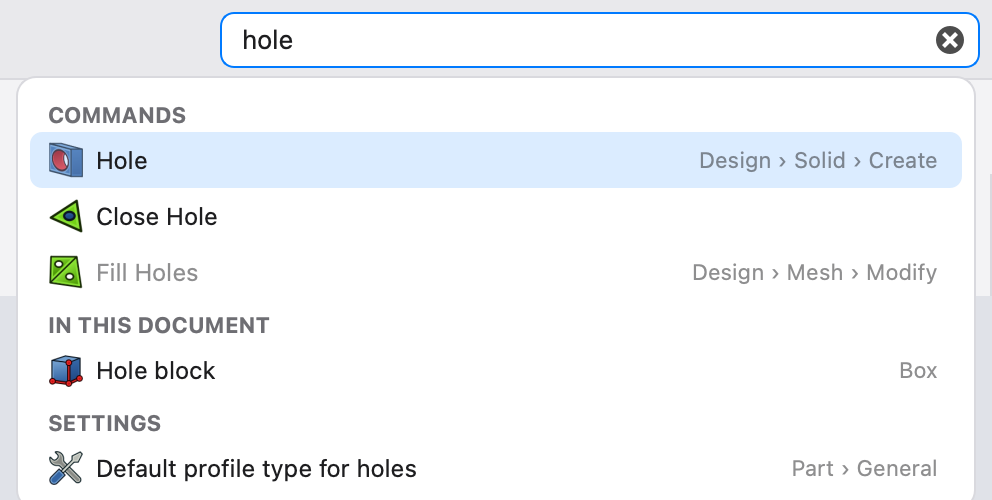
\includegraphics[height=7.2cm,trim=0 0 0 0,clip]{fig/ui_stepC_built_search.png}
\caption{\emph{Left (C1):} the \textsc{Create} caption's menu, the row's commands, then \textsc{More in this group}
from \file{workspaces.json}. \emph{Right (C3):} ``hole'' in the search field, in the title row. Fill Holes is grey:
it needs a mesh selected. Return on the setting opens Preferences at that setting.}
\label{fig:stepC-built-menus}
\end{figure}

\paragraph{C1. Captioned tool groups (done).} \file{bruceworx\_groups.py} gives every workbench toolbar in the
top area a 14\,px bottom margin with a flat caption button in it (\textsc{Create}~$\blacktriangledown$), centred
under the buttons, and a thin divider after each group. The caption's menu holds the toolbar's own
\code{QAction}s under a small \textsc{Create} heading, so enabled and checked states and shortcuts are live; the
workspace's ``more'' commands follow under \textsc{More in this group} (figure~\ref{fig:stepC-built-menus}). Stock
toolbars get short captions (\textsc{Construct}, \textsc{Create}, \textsc{Modify}, \textsc{Pattern} for Part
Design; Sketcher's edit toolbars \textsc{Sketch}, \textsc{Create}, \textsc{Constrain}, \textsc{Modify},
\textsc{Display}); other titles lose their workbench prefix. App toolbars, floating and vertical toolbars get no
caption. Switch: \emph{Captioned tool groups}. 13 tests.

\paragraph{C2. Workspaces and tabs (done).} \file{workspaces.json} defines Design (Part Design: \textsc{Solid},
\textsc{Surface}, \textsc{Mesh}, \textsc{Utilities}), Simulation (FEM), Manufacture (CAM) and Drawing (TechDraw),
\texttt{Cmd-1}\ldots\texttt{4}. At start-up \file{bruceworx\_workspaces.py} writes one FreeCAD custom toolbar per
group (\code{BaseApp/Workbench/PartDesignWorkbench/Toolbar/BW\_*}, named ``Solid~$\cdot$~Create''); a workbench
manipulator takes out the four stock Part Design toolbars and the stock workbench selector while the bar is on.
Commands from other workbenches (Part, Surface, Mesh, Assembly) load through \file{bruceworx\_wsload.py}, which
the custom toolbars name as their module: all 121 commands in the file resolve. The \textsc{Sheet Metal} tab is not
there yet: the add-on is not installed here, so its command names could not be checked; it comes when the
add-on is bundled. Changing tabs only shows and hides toolbars. Opening a sketch adds an accent \textsc{Sketch} tab with Sketcher's edit toolbars and a
\textsc{Finish Sketch} button; finishing returns to the last tab. A workbench chosen from \emph{More workbenches}
gets one tab with its own toolbars. \emph{Choose workbenches\ldots} opens the stock Workbenches page, which is the
one list of enabled workbenches (question~5). The Assembly workbench adds nothing to the context menu (its
\code{ContextMenu} is empty) and its task-panel lists are off, so staying on Part Design loses nothing
(question~3). Switch: \emph{Workspaces and tabs}; off gives back the stock toolbars and selector. 16 tests (the
definition, the parameter writer, the rows).

\paragraph{C3. Search, \texttt{Cmd-K} (done).} \file{bruceworx\_search.py}: one field (in the title row with C4,
otherwise on the first toolbar row). \texttt{Cmd-K} focuses it from anywhere; no FreeCAD command used
\texttt{Ctrl+K}. Results come in three sections (figure~\ref{fig:stepC-built-menus}): commands with their place
(\textsc{Design $\rightarrow$ Solid $\rightarrow$ Create}) or shortcut, active ones first; objects in the active
document; settings, from \file{settings\_index.json} (1\,083 labels of 19 areas, made from the preference pages'
\file{.ui} files by \file{make\_settings\_index.py}). Ranking: whole text, word start, anywhere, letters in
order; tooltips count half, recent use breaks ties; weak hits are dropped when there are enough strong ones.
\texttt{Return} runs, selects or opens Preferences with the text in its own search box, which jumps to the page
and highlights the setting. \texttt{Cmd-Return} on a command opens its workspace and tab and flashes the button.
The SearchBar add-on's toolbar is hidden while the field is on. Switch: \emph{Search field (Cmd-K)}. 12 tests.
Found while building: \code{Command.isActive()} crashes FreeCAD for some commands that are asked outside their
context, so search reads the state of the command's own button instead.

\paragraph{C4. Document tabs in the title bar (done, macOS).} \file{bruceworx\_titlebar.py} makes the window's
content full size with a transparent, untitled title bar, through the Objective-C runtime from \code{ctypes} (no
compiled code). An empty compact \code{NSToolbar} makes the strip 40\,pt: the traffic lights then sit centred at
$x = 12$--$72$, measured on this Mac, so the 40\,px row of the mock works without moving them (question~6). The
row (\code{BruceWorxTitleRow}) has save, undo and redo, the document tabs with the step~B dot, a \emph{+} for a
new document, and the search field on the right. Its tabs mirror the document area's own tab bar, which is hidden
and styled to zero height so its space is given back; clicks, closing and dragging are passed back to it. A press
on empty row space moves the window; a double-click zooms or minimises as System Settings says. Qt's unified
title bar is off while the row is on (\code{MainWindow/UnifiedTitleAndToolBar}, restored afterwards). The
workspace bar now shares row~2 with File and View. Switch: \emph{Document tabs in the title bar}; off brings back
the title bar and step~B's tab row. 5 tests. Found while building: Qt keeps the old title strip as a safe area for every
widget, so each widget in the row has \code{WA\_ContentsMarginsRespectsSafeArea} off; so do the docks, because a
dock laid out while the window changed (the floating Browser before the first document opens) kept its tree
outside its card, and the timeline dock warned about negative sizes. Full screen checked: the
inset drops to 8\,px and comes back. Not checked yet: Stage Manager, dragging and double-clicking the row by
hand, and a capture of the native window (macOS refused window captures while the screen was
locked; the figures are Qt grabs, without the traffic lights).

\paragraph{C5. Start page (done).} \file{bruceworx\_start.py} adds its page to the stock Start view's page
stack and selects it, again whenever \textsc{Start} is reopened or the stock view switches pages itself; switching
it off shows the stock page (question~7: the vault homepage replaces the stock page). Left: \emph{New} (Part,
Assembly, Drawing, Sketch, Simulation study, doing what the stock buttons do), \emph{Open file\ldots} and
\emph{Import STEP / STL\ldots}, then the vault box: ``No vault open'' with \emph{Open vault\ldots} until a vault is
set (\code{BruceWorx/VaultPath}), then the vault's counts. Right: recent files as cards with the thumbnail from
inside each \file{.FCStd}, filters (All, Parts, Assemblies, Drawings) and a name or part-number filter, then a table
with part number, revision, state, date and location, read from each file's \file{Document.xml} on a worker
thread and cached by modification time. At the foot: the stock examples and \emph{Show this page at startup}.
Checked in light and dark, with the switch off and on, and after closing and reopening Start
(figure~\ref{fig:stepC-built-start}). Switch: \emph{BruceWorx Start page}. 21 tests.

\begin{figure}[!htbp]
\centering
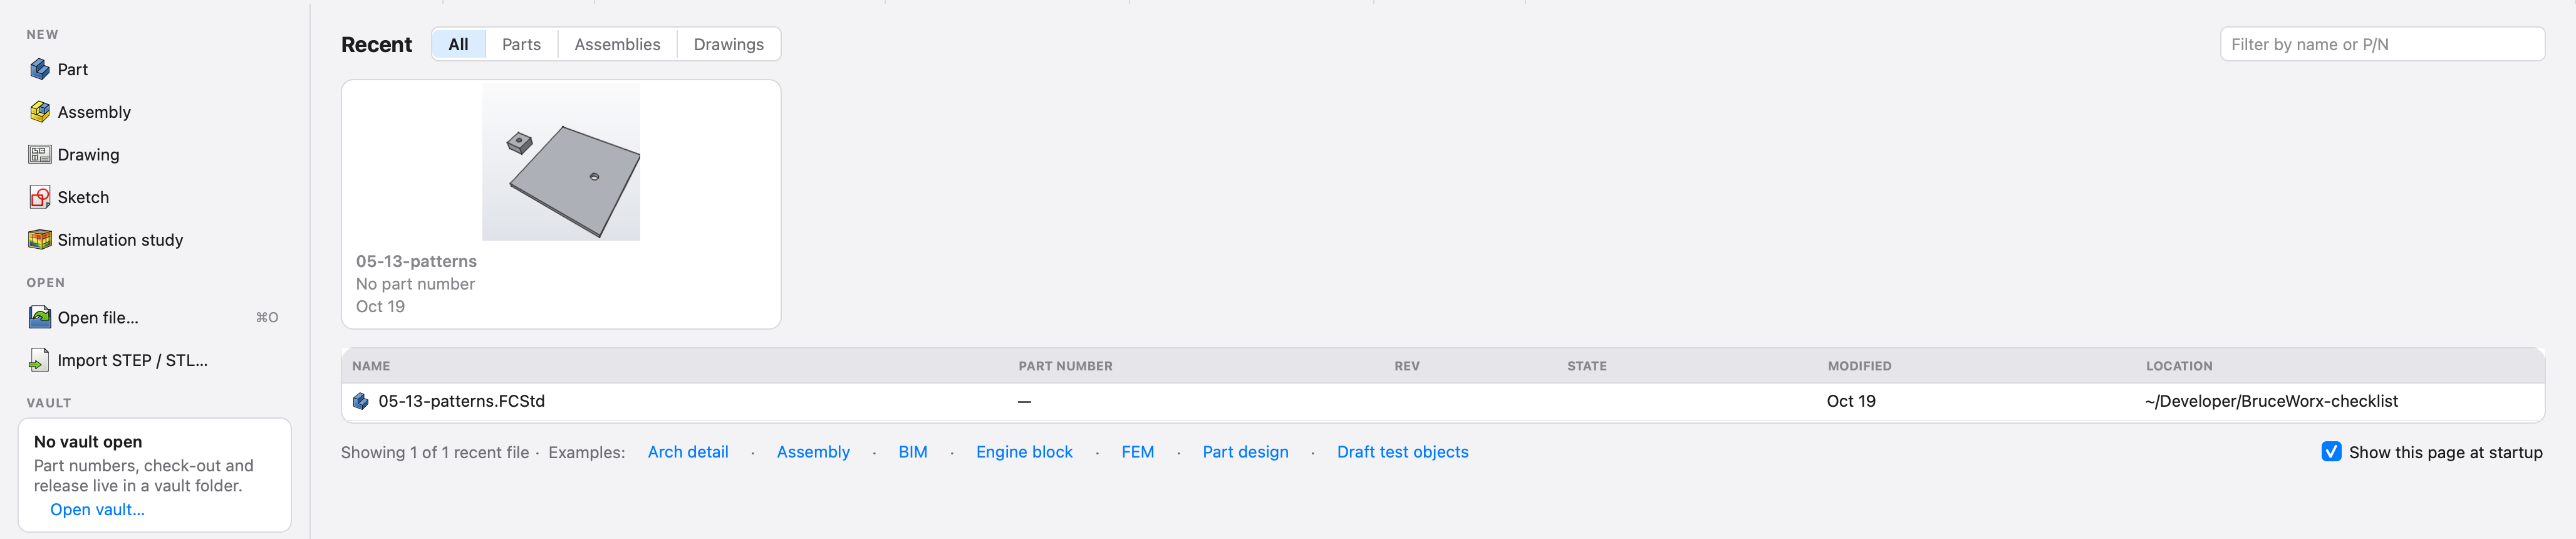
\includegraphics[width=\linewidth]{fig/ui_stepC_built_start.png}\\[4pt]
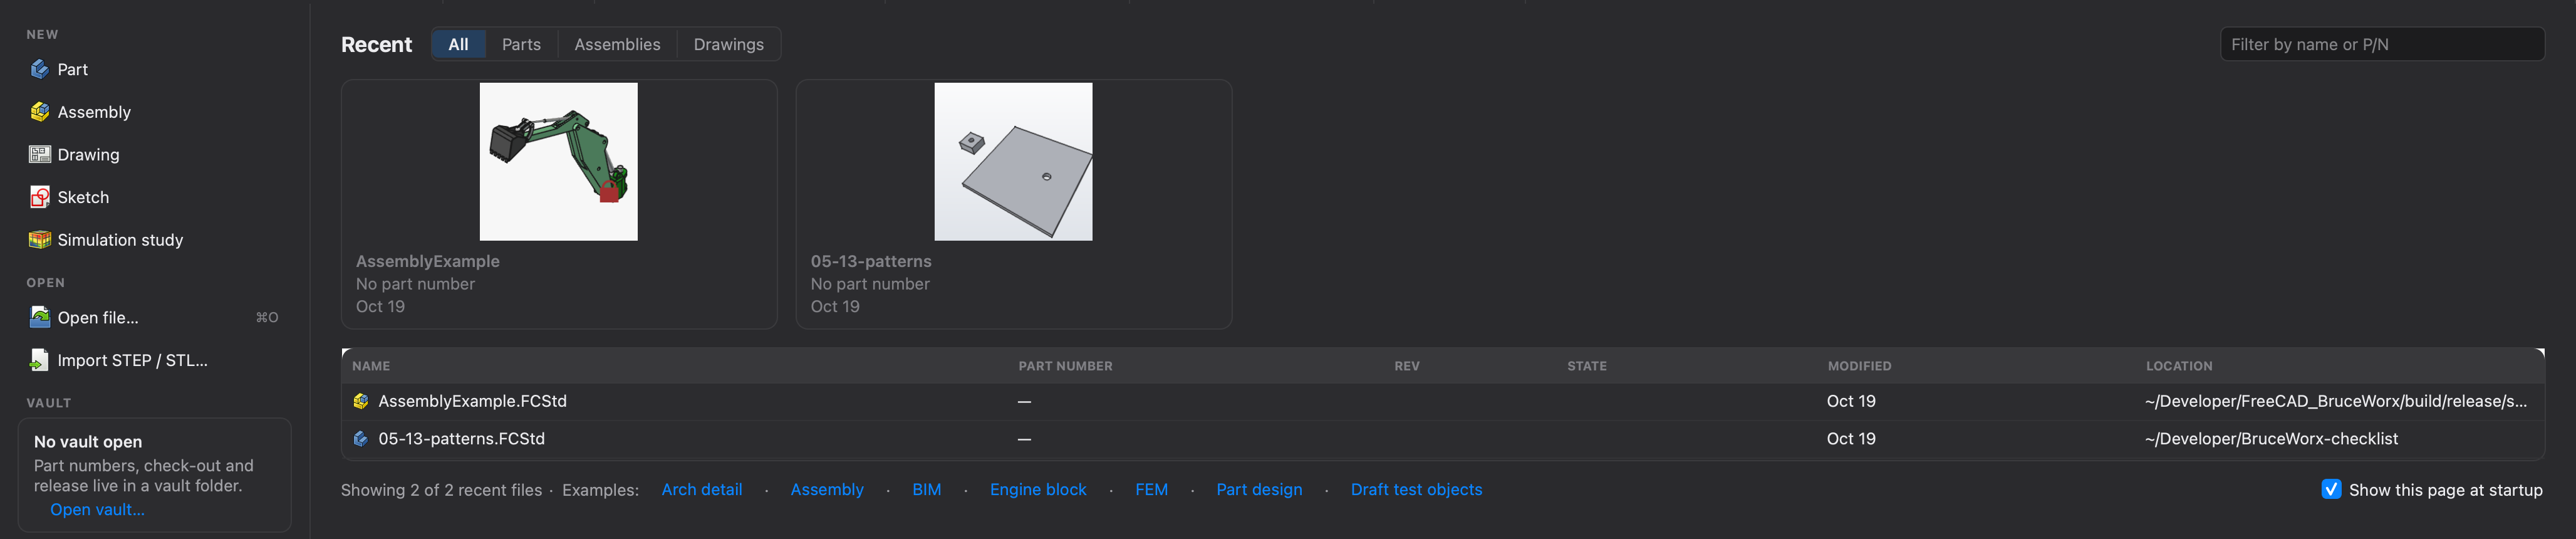
\includegraphics[width=\linewidth]{fig/ui_stepC_built_start_dark.png}
\caption{C5: the Start page as built, light and dark (Qt captures of the build, test configuration with two
recent files and no vault).}
\label{fig:stepC-built-start}
\end{figure}

\paragraph{Checklist for step C.} Re-apply the BruceWorx pack first (it now sets \emph{Drag at cursor} and locks
the toolbars), then restart.
\begin{center}
\small
\begin{longtable}{@{}p{0.6cm}p{6.3cm}p{6.6cm}c@{}}
\toprule
\# & Do & Expect & OK\\
\midrule\endhead
\bottomrule\endfoot
C1 & Look at the window's top edge. & One row: traffic lights, save/undo/redo, document tabs, \emph{+}, the search
  field on the right; no title strip and no tab row under the toolbars. & \tick\\
C2 & Drag the empty part of that row; double-click it. & The window moves; the double-click zooms (or does what
  System Settings says). & \tick\\
C3 & Open two files, edit one, click between the tabs, drag a tab, close one with its \(\times\). & The edited
  one shows a dot; clicks switch documents; the order follows the drag; close asks to save if needed. & \tick\\
C4 & Click \textsc{Design} $\blacktriangledown$; press \texttt{Cmd-2}, then \texttt{Cmd-1}. & The menu lists
  four workspaces with \texttt{Cmd-1}\ldots\texttt{4}; Simulation opens FEM with one tab; Design comes back. & \tick\\
C5 & In Design, click \textsc{Surface}, \textsc{Mesh}, \textsc{Utilities}, \textsc{Solid}. & Only the tools
  change, no flicker; each group has a caption. & \tick\\
C6 & Click the \textsc{Create} caption. & A menu with the row's commands, then \textsc{More in this group} (Groove,
  Subtractive\ldots). & \tick\\
C7 & Start a sketch, draw a line, press \textsc{Finish Sketch}. & A blue \textsc{Sketch} tab and the button appear
  while editing, with Sketcher's groups; afterwards the last Design tab is back. & \tick\\
C8 & \texttt{Cmd-K}, type \emph{hole}; arrow down; Return. Then \emph{smooth} and \texttt{Cmd-Return}. & Hole runs
  (with a face selected); \texttt{Cmd-Return} opens \textsc{Mesh} and flashes Smooth. & \tick\\
C9 & \texttt{Cmd-K}, \emph{profile type for holes}, Return. & Preferences open on Part $\rightarrow$ General with
  the setting highlighted. & \tick\\
C10 & Preferences $\rightarrow$ BruceWorx: untick, one at a time, \emph{Document tabs in the title bar},
  \emph{Workspaces and tabs}, \emph{Captioned tool groups}, \emph{Search field}; tick them again. & Each gives back
  the stock look on its own and comes back when ticked. & \tick\\
C11 & Open the \textsc{Start} tab; click a recent card, the \emph{Parts} filter, then \emph{New} $\rightarrow$
  Part. & Cards and table show your recent files with thumbnails; the card opens its file; New Part opens a body. & \tick\\
\end{longtable}
\end{center}

\paragraph{6. Create Vault wizard (23 Oct, built straight away at your request).} You asked for a wizard covering
name and location (iCloud Drive by default), part numbering in the fixed form (an editable form later), company part
properties and the import of existing files. BruceWorx $\rightarrow$ \emph{Create Vault\ldots} (also in
\texttt{Cmd-K}), the Start page's \emph{Create vault\ldots} link, and \emph{Open vault\ldots} on a folder that is not a
vault all open a five-step dialog with the steps listed on the left (figure~\ref{fig:vault-wizard}): name and location
(the folder follows the name inside iCloud Drive's ``BruceWorx Vaults'' until you type one; problems shown as you
type), part numbering (programs, two-digit document types, first parent number and revision, with a live example
such as \texttt{BW-01-01001-001-A}), company part properties (MaterialSpec, HeatTreatment, ToleranceClass, Customer,
Project, or your own text, whole-number or list properties), a summary with \emph{Create} and \emph{make this the
open vault}, and an optional import. The engine is \file{bruceworx/vault\_setup.py} in the hooks add-on, also behind
\texttt{bw-hooks vault init} and \texttt{vault import --from <folder> [--dry-run]}. A new vault holds
\file{numbering.json}, \file{document\_types.json} and \file{part\_properties.json} next to its ref file; while it is
the open vault its numbering drives \emph{Assign Part Number} and its properties are a schema layer. Import reads
each file's \file{Document.xml} without FreeCAD, classifies it as part, assembly or drawing, previews numbers without
reserving them, keeps valid existing part numbers, and checks in a numbered copy: the originals are never changed
(tested byte for byte). 26 engine tests and 14 dialog tests; a test vault was created and the six checklist files
imported in light and dark. Open questions are in the answer to you, not repeated here.

\begin{figure}[!htbp]
\centering
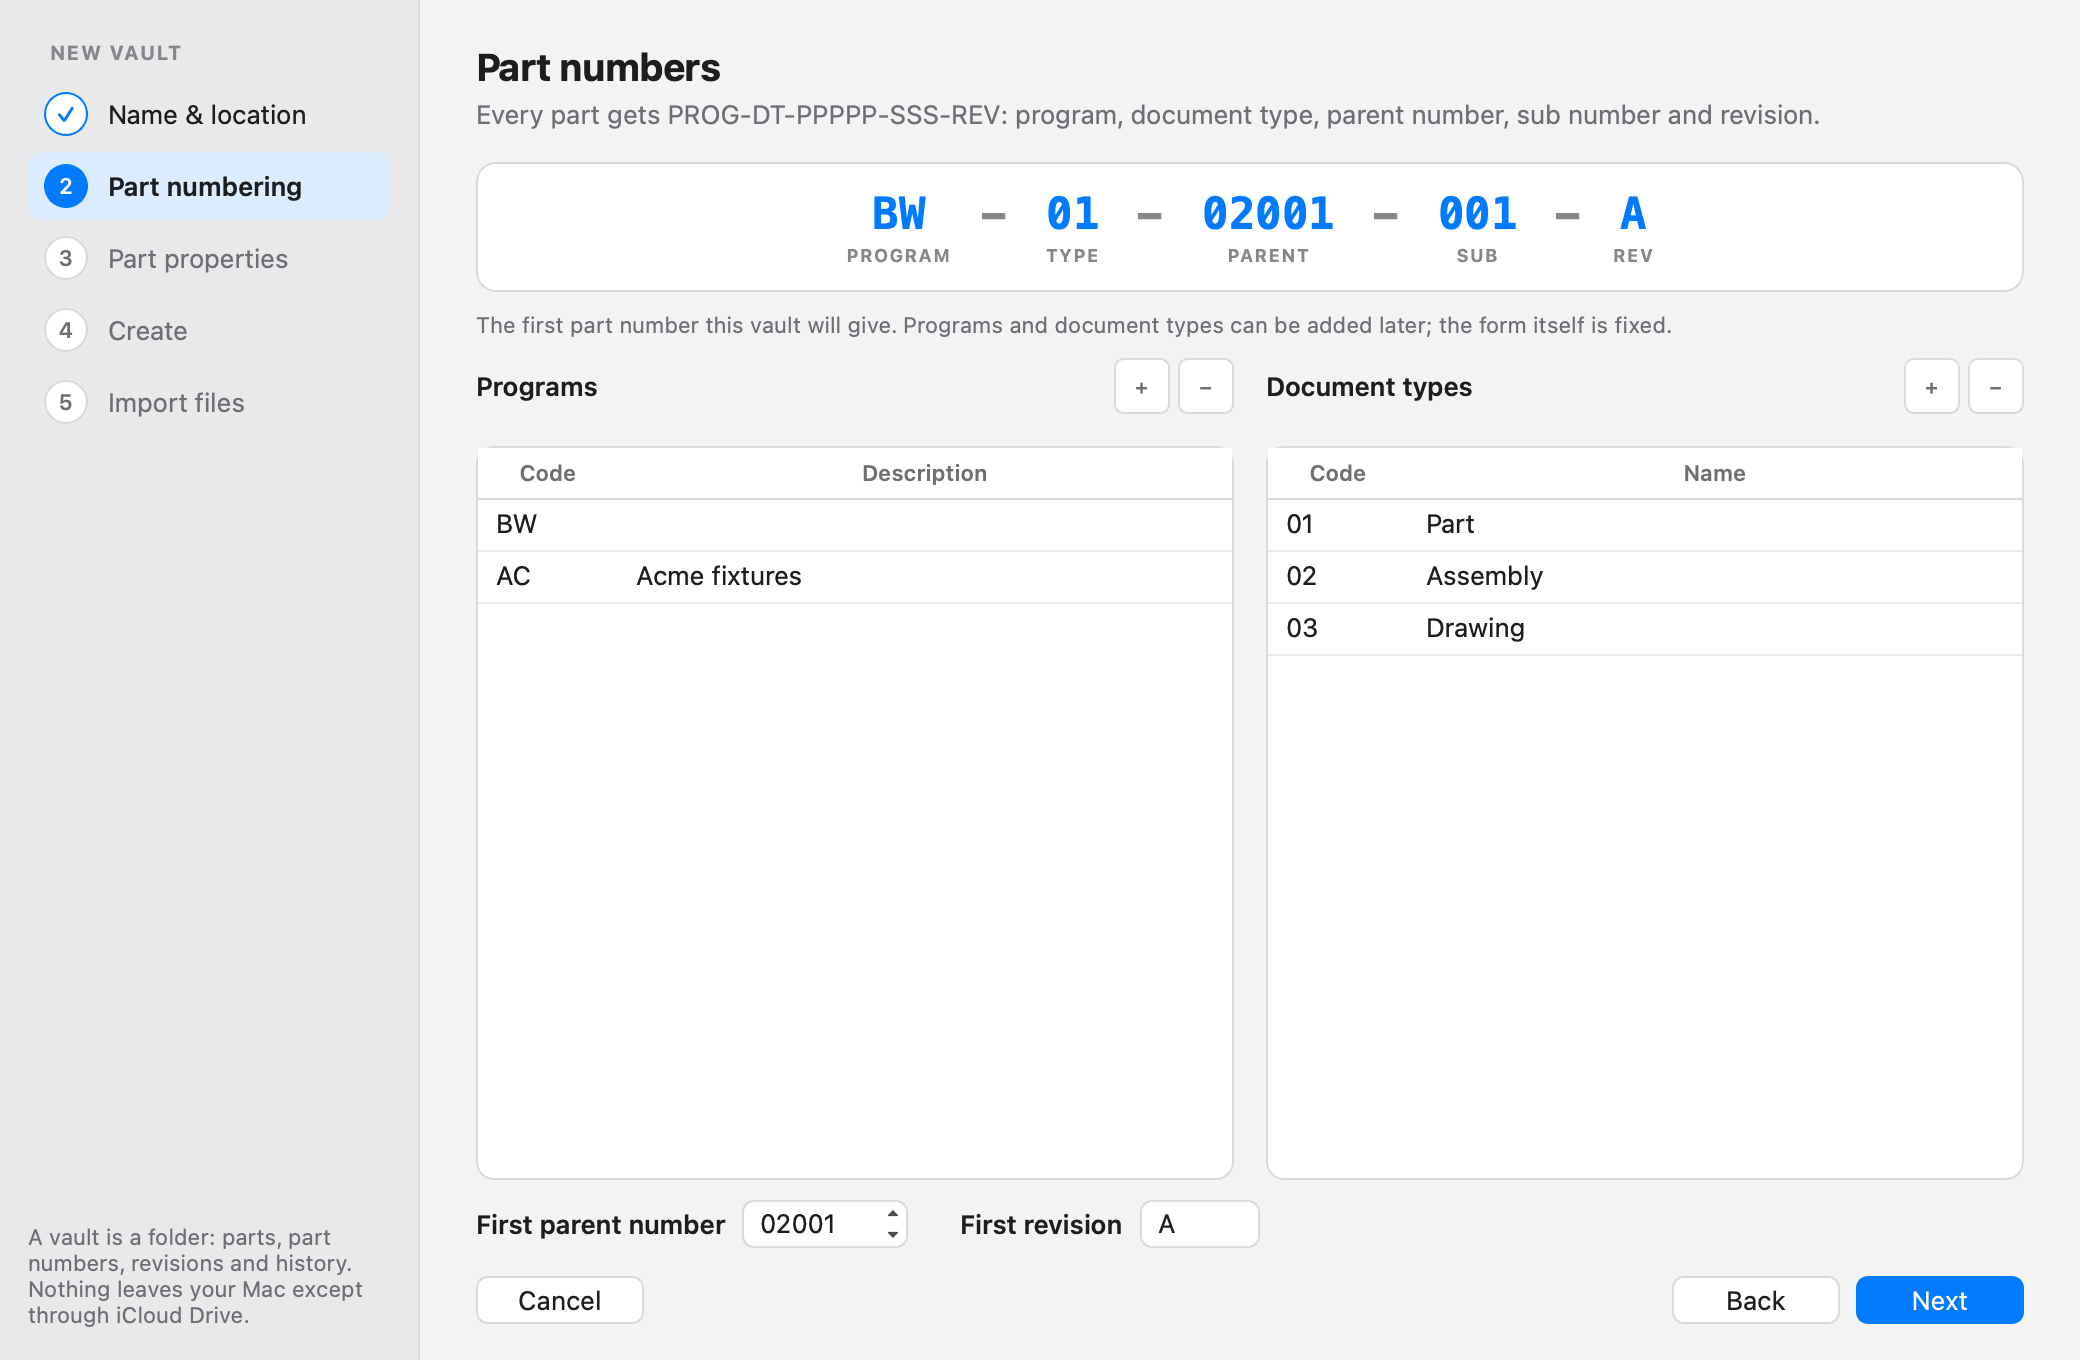
\includegraphics[width=0.497\linewidth]{fig/vault_wizard_numbering.png}\hfill
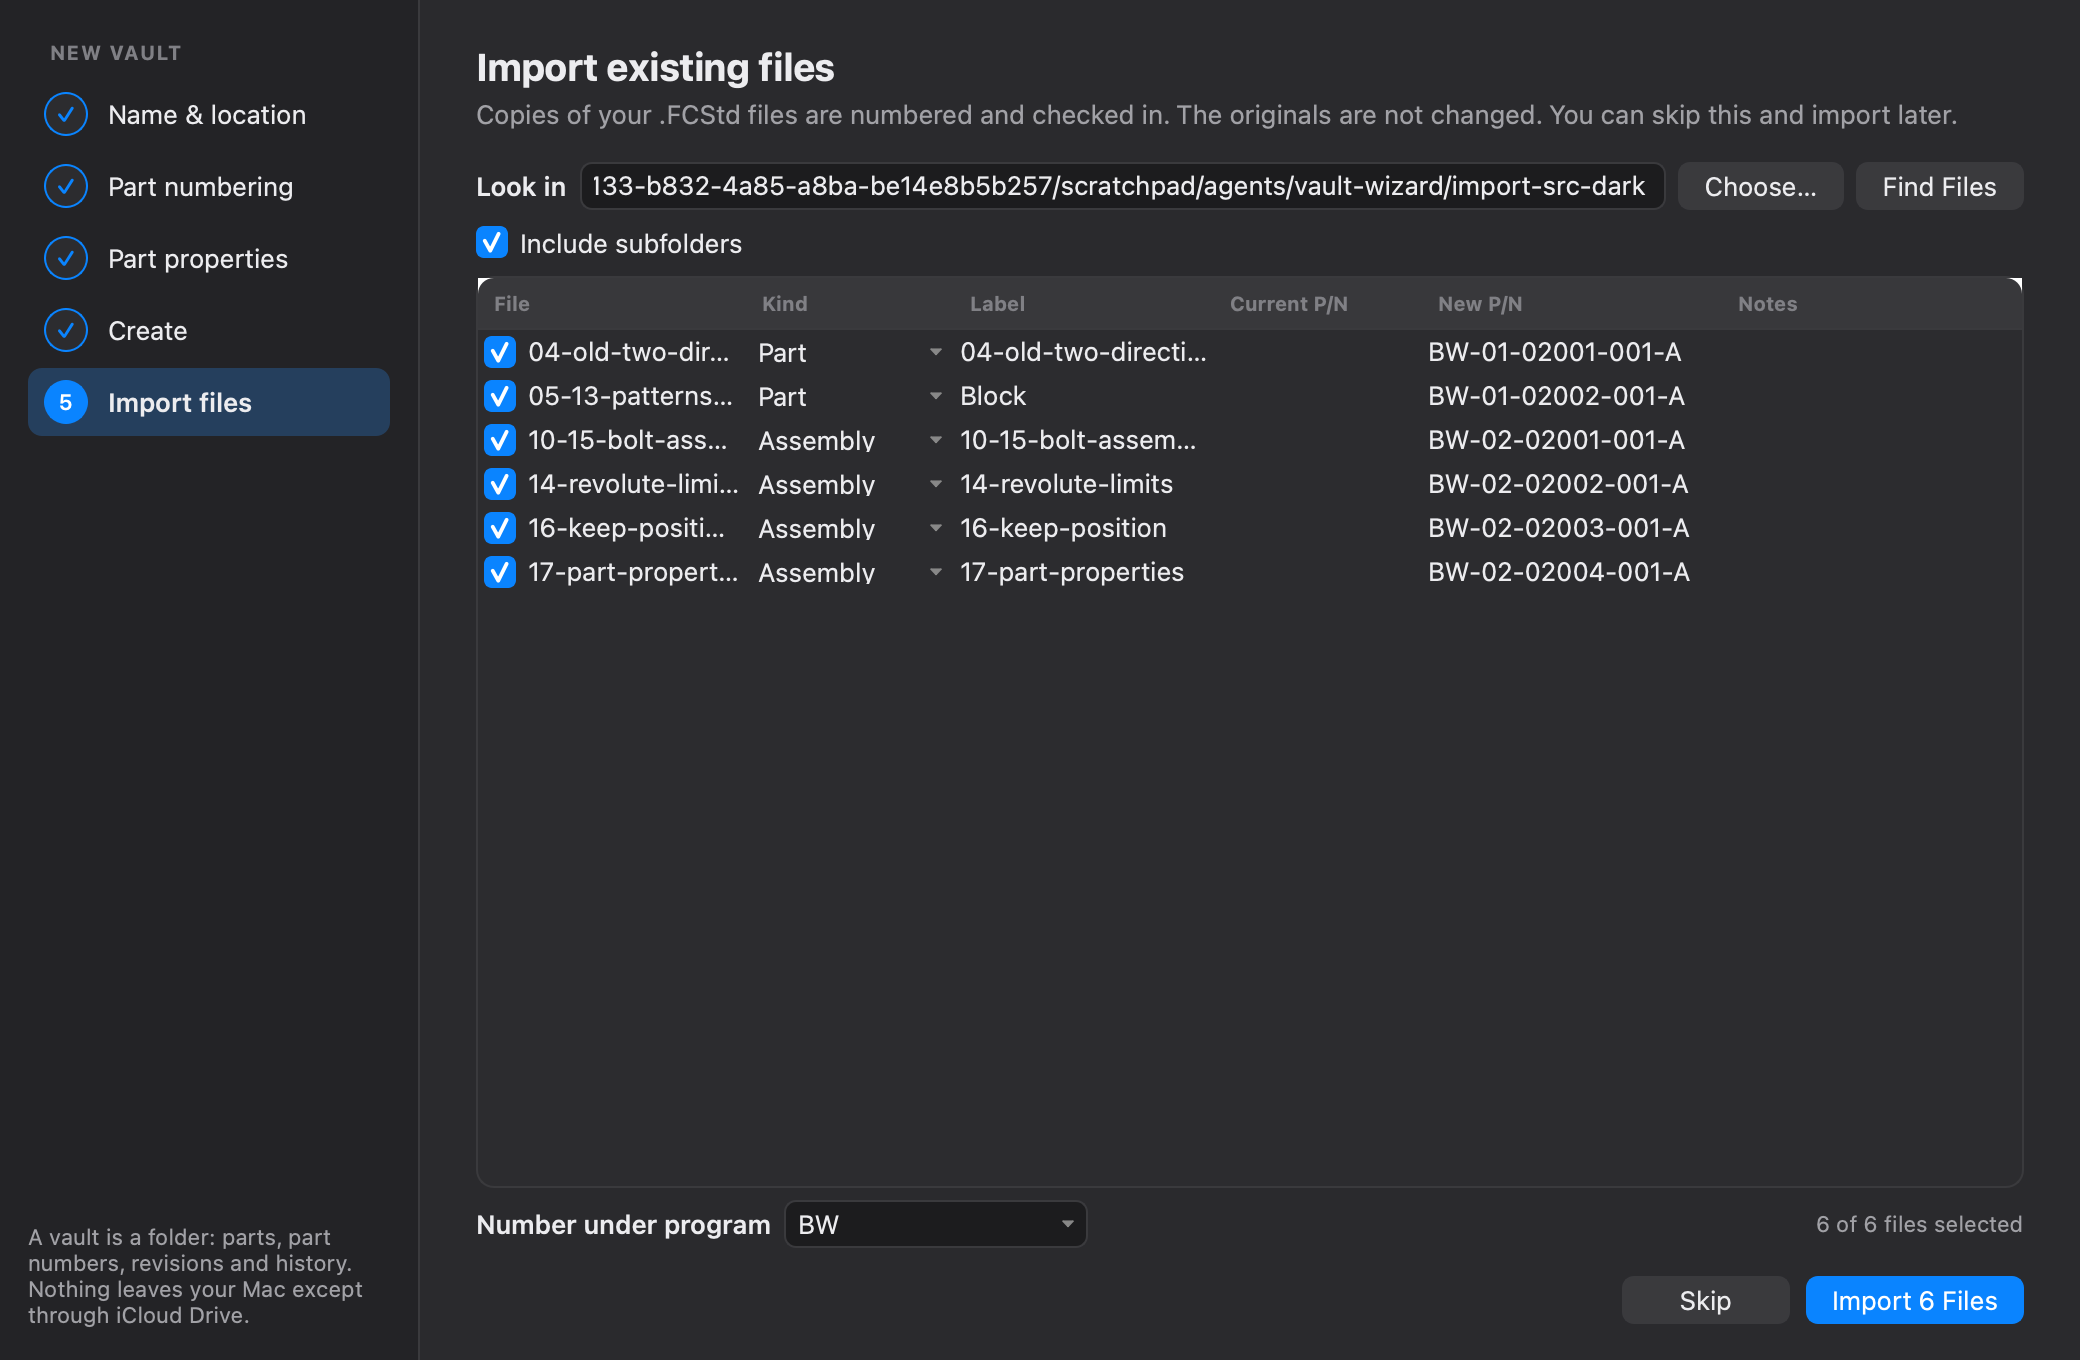
\includegraphics[width=0.497\linewidth]{fig/vault_wizard_import_dark.png}
\caption{Create Vault: the numbering step (light) and the import step with six files found (dark).}
\label{fig:vault-wizard}
\end{figure}

\paragraph{7. Fixed along the way.} The notification pop-up was see-through (the stylesheet's \code{QLabel} rule
reached it), so the navigation pill showed through: it is now named before it is styled (\code{[BW]} in
\file{NotificationBox.cpp}) and has a solid card. The pack no longer asks for the view cube font ``Noto Sans'',
which macOS does not have and which made Qt warn on every start.
